
\section{Introduction}

À la suite de l’analyse des besoins, la phase de conception vise à établir la structure logique et le fonctionnement global du système. Elle traduit les exigences fonctionnelles et non fonctionnelles en une architecture cohérente, mettant en évidence les principaux composants, leurs interactions et les flux d’informations qui les relient. Cette étape garantit que la solution répond aux attentes des utilisateurs tout en respectant les contraintes de performance, de fiabilité et de sécurité. Les modèles UML présentés dans cette section (cas d’utilisation, activités, classes et séquences) reflètent les choix de conception effectués en vue de la réalisation de la plateforme.


\section{Objectifs de conception}
La conception de RevMine vise à proposer une solution capable de regrouper l’ensemble du processus d’analyse des données de revue de code dans une plateforme accessible, efficace et conviviale. Les objectifs retenus orientent les choix architecturaux et permettent d’assurer l’adéquation entre les besoins identifiés et la solution proposée.

\vspace{0.5cm}

\begin{tabularx}{\textwidth}{|l|X|}
\hline
\textbf{Objectif} & \textbf{Description} \\ \hline

\textbf{Accessibilité} & Permettre à différents profils d’utilisateurs, notamment les chercheurs, praticiens DevOps et managers, d’exploiter les données de revue de code sans nécessiter une expertise avancée en programmation ou en manipulation d’API. \\ \hline

\textbf{Modularité} & Séparer les principales responsabilités du système en modules indépendants, tels que la gestion des espaces de travail, la collecte, l’analyse et la visualisation, l’interaction avec les modèles de langage. \\ \hline

\textbf{Maintenabilité} & Faciliter l’évolution et la correction du système en permettant la modification d’un module sans impacter l’ensemble de la plateforme. \\ \hline

\textbf{Extensibilité} & Permettre l’ajout progressif de nouvelles plateformes, métriques, analyses et modèles LLM afin d’adapter RevMine à l’évolution rapide du domaine. \\ \hline

\textbf{Fiabilité} & Garantir une collecte correcte et robuste des données, en limitant les risques d’erreurs, de pertes de données ou d’interruptions non maîtrisées. \\ \hline

\textbf{Réutilisabilité des données} & Conserver les données collectées et l’historique des opérations afin d’éviter les collectes répétées et de permettre des analyses ultérieures. \\ \hline

\textbf{Sécurité} & Assurer la protection des informations sensibles, notamment les tokens d’accès aux plateformes Git ainsi que les données collectées à partir des projets. \\ \hline

\textbf{Flexibilité} & Offrir à l’utilisateur la possibilité d’utiliser différents fournisseurs de modèles de langage, y compris des modèles locaux, afin de répondre aux contraintes de confidentialité, de coût ou de performance. \\ \hline

\end{tabularx}

\vspace{0.5cm}

Ces objectifs constituent la base des décisions de conception adoptées pour RevMine.


\section{Architecture générale}
\subsection{Étude comparative des styles architecturaux}

Les architectures logicielles contemporaines les plus répandues incluent les approches monolithique, modulaire, microservices et serverless. Chacune présente des compromis entre flexibilité, complexité et performance. Le Tableau suivant résume les principales caractéristiques de ces modèles architecturaux selon la littérature récente.



\begin{table}[H]
\centering
\small
\begin{tabularx}{\textwidth}{|l|Y|Y|Y|Y|Y|}
\hline
\textbf{Architecture} & \textbf{Scalabilité} & \textbf{Extensibilité} & \textbf{Résilience} & \textbf{Complexité de déploiement} & \textbf{Cas d’usage typiques} \\
\hline
Monolithique & Faible à moyenne, principalement verticale & Limitée par le couplage interne & Faible à moyenne & Faible & Applications simples, stables ou de petite taille \\
\hline
Modulaire & Moyenne & Moyenne à élevée & Moyenne & Moyenne & Applications structurées en composants fonctionnels séparés \\
\hline
Microservices & Élevée, principalement horizontale & Élevée grâce à l’indépendance des services & Élevée & Élevée & Systèmes distribués, évolutifs et nécessitant plusieurs traitements indépendants \\
\hline
Serverless & Très élevée & Moyenne & Élevée & Moyenne & Traitements ponctuels, événementiels ou temporaires\\
\hline
\end{tabularx}
\caption{Comparaison des principales architectures logicielles selon la littérature.}
\label{tab:comparaison_architectures}
\end{table}

Cette comparaison montre que chaque architecture présente des avantages et des limites selon le contexte d’utilisation. L’architecture monolithique se distingue par sa simplicité de développement et de déploiement, mais elle devient moins adaptée lorsque le système évolue ou lorsque les composants doivent être modifiés indépendamment \cite{richards2015software}. Les architectures modulaires améliorent l’organisation interne du système, mais elles ne garantissent pas toujours une mise à l’échelle indépendante des composants \cite{richards2015software}. Les microservices, quant à eux, permettent de découper le système en services autonomes, faiblement couplés et indépendamment déployables, ce qui favorise la scalabilité, la maintenabilité et l’évolution continue du système \cite{fowler2014microservices,newman2021building}. Fowler et Lewis décrivent les microservices comme des services indépendamment déployables et scalables, avec des frontières modulaires claires \cite{fowler2014microservices}. IBM souligne également que les microservices offrent une meilleure scalabilité que les architectures monolithiques, notamment parce que les services peuvent être mis à l’échelle séparément \cite{ibm2024monolithicMicroservices}. Toutefois, cette approche introduit une complexité plus importante, notamment en matière de coordination, de communication et de gestion globale du système \cite{richards2015software,newman2021building}. Enfin, l’architecture serverless est adaptée aux charges variables et événementielles, mais elle dépend fortement des plateformes cloud et présente encore plusieurs défis techniques, notamment autour de la gestion de l’état et de la prévisibilité des performances \cite{baldini2017serverless}.

\subsection{Choix architectural}

À la suite de la définition des objectifs de conception et de l’étude comparative des principaux styles architecturaux, l’architecture \textbf{Microservices organisée en couches} apparaît comme le choix le plus adapté pour RevMine.

Ce style architectural permet de répondre aux exigences principales du système, notamment la séparation des responsabilités, l’évolutivité, la maintenabilité et l’intégration de composants hétérogènes tels que les services de collecte, d’analyse, de stockage et d’interaction avec les modèles de langage.

Ainsi, ce choix architectural sera retenu pour la conception de RevMine. La section suivante présente les éléments qui justifient plus en détail cette décision.



\subsection{Justification du choix}

Le choix d’une architecture microservices organisée en couches se justifie par la nature même de RevMine, dont les principales fonctionnalités correspondent à des responsabilités distinctes. La gestion des workspaces et des dépôts, la collecte des données, l’analyse des résultats et l’interaction en utilisant le language naturel peuvent être considérées comme des domaines fonctionnels relativement indépendants.

Cette architecture permet ainsi de répondre aux objectifs de conception définis précédemment :

\begin{itemize}
    \item \textbf{Accessibilité} : la séparation entre l’interface utilisateur, les services de traitement et les services d’analyse permet de proposer une plateforme claire et exploitable par différents profils d’utilisateurs.

    \item \textbf{Modularité et maintenabilité} : chaque service porte une responsabilité précise, ce qui facilite son évolution, sa correction ou son remplacement sans affecter l’ensemble du système.

    \item \textbf{Extensibilité} : l’ajout de nouvelles plateformes, métriques, analyses ou modèles LLM peut être réalisé progressivement, en intervenant uniquement sur les services concernés.

    \item \textbf{Fiabilité} : l’isolation des traitements, notamment ceux liés à la collecte des données, permet de mieux gérer les erreurs et de limiter leur impact sur le reste de la plateforme.

    \item \textbf{Réutilisabilité des données} : les données produites par chaque service peuvent être conservées dans son propre espace de persistance, ce qui permet de réutiliser les résultats de collecte, de structuration ou d’analyse sans répéter inutilement les mêmes opérations.
\end{itemize}

Ainsi, l’architecture retenue permet d’aligner la structure technique de RevMine avec sa logique fonctionnelle. Elle offre une base adaptée pour construire une solution évolutive, maintenable et cohérente avec les besoins identifiés.

\section{Vue initiale de l’architecture de RevMine}
La figure ci-dessous présente une vue initiale et simplifiée de l’architecture de RevMine. Elle met en évidence les principales couches de la solution, à savoir la couche de présentation, l’API Gateway, les microservices, la couche de persistance, les services externes ainsi que les mécanismes de communication et de mise en cache. Cette représentation permet d’avoir une première vision globale de l’organisation du système avant de détailler chaque service séparément.
\vspace{1em}
  \begin{figure}[H]
            \centering
            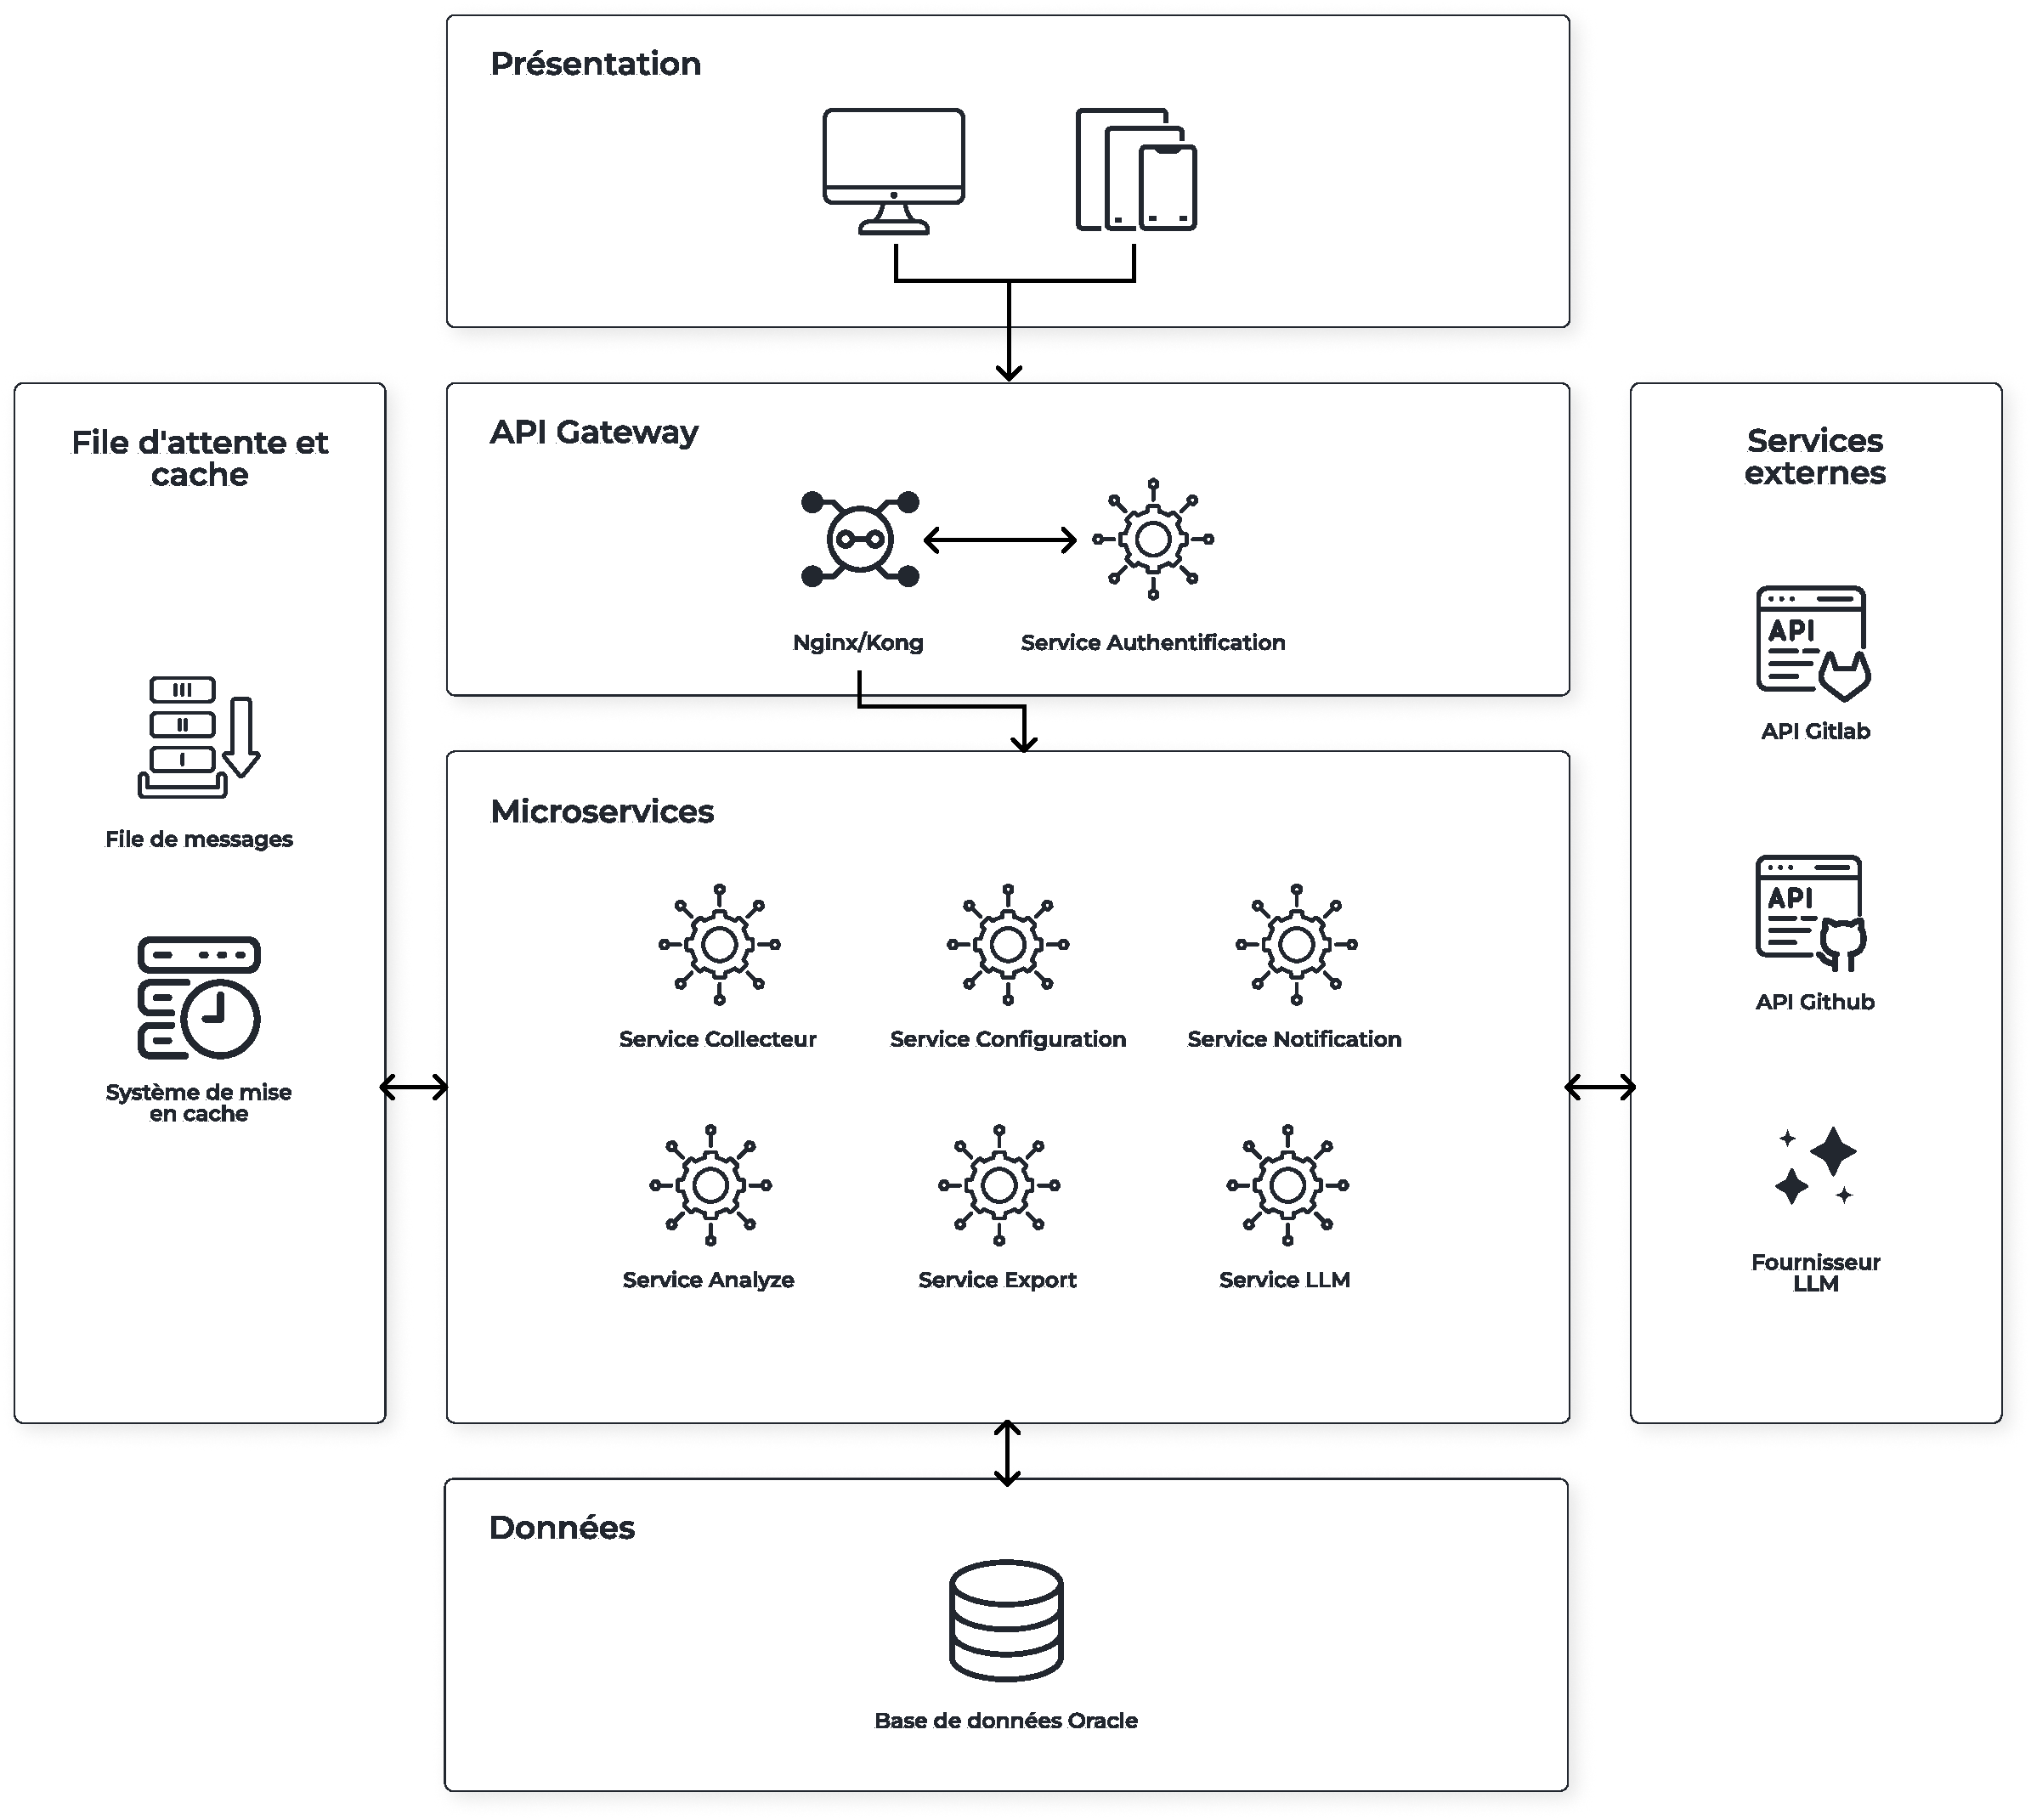
\includegraphics[width=\textwidth]{figures/diagramm_architecture_p.pdf}
            \caption{Schéma simplifié de l’architecture générale de la solution.}
            \label{fig:architecture_generale}
        \end{figure}

\vspace{1em}
L’architecture est structurée autour des éléments suivants :

\begin{itemize}
    \item \textbf{Couche présentation :} elle correspond à l’interface utilisateur de RevMine. Il s’agit d’une interface web intuitive permettant aux utilisateurs d’effectuer les principales opérations offertes par la plateforme, notamment la configuration des projets, le lancement des collectes, l’analyse des données et la consultation des résultats.

    \item \textbf{API Gateway :} cette couche constitue le point d’entrée principal du système. Elle reçoit les requêtes provenant de l’interface utilisateur et les redirige vers les services appropriés. Elle joue également un rôle important dans la gestion de l’authentification et du contrôle d’accès, afin d’assurer que seules les requêtes autorisées soient traitées.

    \item \textbf{Microservices :} cette couche regroupe les services contenant la logique métier de la solution. Chaque service est responsable d’un périmètre fonctionnel précis :
    \begin{itemize}
        \item \textbf{Service de configuration :} permet la connexion aux plateformes GitHub et GitLab, la gestion des tokens, ainsi que l’importation et la gestion des dépôts à analyser.

        \item \textbf{Service collecteur :} prend en charge la configuration et l’exécution des collectes de données de revue de code. Il gère également les opérations associées aux données collectées, telles que le nettoyage, le filtrage, l’historique des collectes et des traitements, ainsi que le calcul des métriques nécessaires à l’analyse.

        \item \textbf{Service d’analyse :} permet d’exploiter les données collectées et les métriques calculées afin de produire différentes analyses, statistiques et visualisations.

        \item \textbf{Service LLM :} assure l’intégration de l’interaction en langage naturel, notamment pour assister l’utilisateur dans la définition des plans de collecte et des analyses.

        \item \textbf{Service de notification :} informe l’utilisateur de l’état des opérations importantes, telles que le démarrage, la progression, la fin ou l’échec d’une collecte ou d’une analyse.

    \end{itemize}

    \item \textbf{Couche données :} bien qu’elle soit représentée de manière regroupée dans le diagramme, cette couche ne correspond pas à une base de données centralisée unique. Dans l’architecture de RevMine, chaque service dispose de sa propre persistance selon ses besoins. En complément, un mécanisme de stockage dédié permet de gérer les fichiers volumineux, tels que les données brutes collectées ou les datasets structurés.

    \item \textbf{Services externes :} RevMine interagit avec des systèmes externes, notamment les API GitHub et GitLab pour l’extraction des données de revue de code, ainsi qu’avec des fournisseurs LLM ou des modèles locaux pour le traitement des requêtes en langage naturel.

    \item \textbf{File d’attente et cache :} ces mécanismes facilitent la communication entre les services, notamment pour les traitements asynchrones ou de longue durée. Ils permettent également d’améliorer la réactivité du système et de mieux gérer certaines opérations répétitives ou coûteuses.
\end{itemize}

Cette vue initiale constitue ainsi une première abstraction de l’architecture de RevMine. Les sections suivantes détaillent la conception interne des différents services afin de mieux comprendre leur structure, leurs responsabilités et les données qu’ils manipulent.

\section{Conception détaillée de l'API Gateway}
L’API Gateway constitue le point d’entrée principal de RevMine. Elle reçoit les requêtes provenant de l’interface utilisateur et les redirige vers les services appropriés. Elle assure également la gestion des utilisateurs, l’authentification, les sessions et la validation des tokens d’accès.

Ce composant joue donc un rôle organisationnel et sécuritaire essentiel, en garantissant la coordination entre l’interface et les différents services métiers.

\begin{table}[H]
\centering
\begin{tabular}{|p{4cm}|p{10cm}|}
\hline
\textbf{Élément} & \textbf{Description} \\
\hline
Entrées & Requêtes utilisateur provenant de l’interface web, informations d’authentification, demandes de routage vers les services. \\
\hline
Sorties & Réponses renvoyées à l’interface utilisateur, tokens de session, requêtes transmises aux services concernés. \\
\hline
Rôle principal & Centraliser l’accès à la plateforme, gérer l’authentification et router les requêtes vers les services métiers. \\
\hline
\end{tabular}
\end{table}

\subsubsection*{Diagramme de classes de l’API Gateway}

Ce diagramme présente les classes liées à la gestion des utilisateurs, des sessions et de l’authentification.
\begin{figure}[H]
\centering

\includegraphics[width=0.9\textwidth]{classDiagramm1.pdf}
\caption{Diagramme de classes de l’API Gateway}
\label{fig:classDiagramm1}
\end{figure}

\section{Conception détaillée des services}
Cette section présente la conception détaillée des principaux services de RevMine. Pour chaque service, nous décrivons son rôle, sa logique fonctionnelle, ses entrées et sorties, ainsi que les besoins fonctionnels auxquels il contribue. Chaque sous-section est complétée par un diagramme de classes et un schéma de base de données afin de préciser la structure interne du service.


\subsection{Service de configuration}

Le service de configuration prépare l’environnement de travail nécessaire aux collectes et aux analyses. Il permet de connecter RevMine aux plateformes GitHub et GitLab, de gérer les tokens d’accès et d’importer les dépôts à analyser.

Les dépôts sont organisés dans des workspaces, ce qui facilite leur gestion, leur sélection et les opérations ultérieures. Ce service assure ainsi la liaison entre RevMine et les plateformes de collaboration logicielle.

\begin{table}[H]
\centering
\begin{tabular}{|p{4cm}|p{10cm}|}
\hline
\textbf{Élément} & \textbf{Description} \\
\hline
\textbf{Entrées} & Tokens d’accès, informations de connexion, paramètres du workspace, dépôts à importer. \\
\hline
\textbf{Sorties} & Workspaces configurés, dépôts importés, métadonnées nécessaires aux collectes. \\
\hline
\textbf{Besoins couverts} & BF1, BF2, BF3, BF4, BF5 \\
\hline
\end{tabular}
\end{table}


\subsubsection*{Diagramme de classes du service de configuration}

Ce diagramme présente les classes liées aux workspaces, aux dépôts et à leur gestion.

\begin{figure}[H]
\centering

\includegraphics[width=0.9\textwidth]{classDiagramm2.pdf}
\caption{Diagramme de classes du service configuration}
\label{fig:classDiagramm2}
\end{figure}


\subsection{Service de collecte}
Le service de collecte permet d’extraire les données de revue de code à partir d’un dépôt sélectionné. La collecte peut être configurée manuellement, en précisant la branche, les endpoints, les filtres, l’état des PR/MR et la plage temporelle, ou générée automatiquement à partir d’un prompt en langage naturel.

Après validation du plan de collecte, le service extrait les données depuis GitHub ou GitLab et les stocke sous forme brute. Il permet ensuite de nettoyer et filtrer ces données afin de produire un dataset structuré, ainsi que de calculer les métriques nécessaires aux analyses futures. Il conserve également l’historique des collectes afin d’éviter les opérations répétitives.

\begin{table}[H]
\centering
\begin{tabular}{|p{4cm}|p{10cm}|}
\hline
\textbf{Élément} & \textbf{Description} \\
\hline
\textbf{Entrées} & Prompt en langage naturel ou configuration manuelle de collecte: dépôt sélectionné, branche, endpoints, filtres, plage temporelle, état des PR/MR. \\
\hline
\textbf{Sorties} & Données brutes collectées, datasets nettoyés et filtrés, fichiers structurés, métriques calculées, historique des collectes. \\
\hline
\textbf{Besoins couverts} & BF6, BF8, BF9, BF10, BF11, BF12, BF13, BF14, BF20, BF22, BF23 \\
\hline
\end{tabular}
\end{table}

\subsubsection*{Endpoints considérés pour la collecte}

Afin de permettre une analyse riche et extensible, le service de collecte est conçu pour prendre en charge différentes familles d’endpoints issues des plateformes GitHub et GitLab. L’objectif est de permettre à l’utilisateur de sélectionner les données pertinentes selon son besoin, tout en conservant la possibilité d’étendre progressivement les métriques calculées.Les principales catégories d’endpoints ciblées sont :
\begin{itemize}    
\item \textbf{Données de revue de code :} pull requests, merge requests, reviewers, auteurs, états, dates de création, fusion et fermeture.    
\item \textbf{Commentaires et discussions :} commentaires généraux, commentaires de revue, discussions et remarques associées aux PR/MR.    
\item \textbf{Commits et changements de code :} commits associés, auteurs, messages, fichiers modifiés, diffs et informations de modification.    
\item \textbf{Métadonnées de projet :} branches, labels, milestones, participants et informations générales du dépôt.    
\item \textbf{Données Kanban :} issues, boards, colonnes, statuts et informations liées au suivi du travail.    
\item \textbf{Données CI/CD :} pipelines, jobs, statuts d’exécution, durées et résultats associés.
\end{itemize}
Cette organisation par familles d’endpoints permet d’adapter la collecte aux objectifs d’analyse, tout en préparant le système à l’ajout de nouvelles métriques ou de nouvelles sources de données.

\subsubsection*{Diagramme de classes du service de collecte}

Ce diagramme présente les classes liées à la configuration, l’exécution, le nettoyage et le suivi des collectes.
\begin{figure}[H]
\centering

\includegraphics[width=0.9\textwidth]{classDiagramm3.pdf}
\caption{Diagramme de classes du service collection}
\label{fig:classDiagramm3}
\end{figure}

\subsection{Service d’analyse}
Le service d’analyse exploite les données collectées et les métriques calculées afin de produire des analyses, statistiques et visualisations. Il peut travailler sur des datasets issus de la collecte interne ou sur des datasets externes importés par l’utilisateur.

L’analyse peut être configurée manuellement, à partir d’analyses prédéfinies, ou automatiquement à partir d’un prompt. Les résultats sont ensuite présentés dans un tableau de bord et peuvent être exportés ou consultés depuis l’historique.

\begin{table}[H]
\centering
\begin{tabular}{|p{4cm}|p{10cm}|}
\hline
\textbf{Élément} & \textbf{Description} \\
\hline
\textbf{Entrées} & Dataset interne ou externe, métriques calculées, configuration manuelle d’analyse ou prompt utilisateur. \\
\hline
\textbf{Sorties} & Analyses, statistiques, visualisations, résultats exploitables, historique des analyses, exports. \\
\hline
\textbf{Besoins couverts} & BF13, BF16, BF17, BF18, BF19, BF20 \\
\hline
\end{tabular}
\end{table}


\subsubsection*{Diagramme de classes du service d’analyse}

Ce diagramme présente les classes liées aux datasets, aux analyses, aux résultats et aux lots d’analyse.
\begin{figure}[H]
\centering

\includegraphics[width=0.9\textwidth]{classDiagramm4.pdf}
\caption{Diagramme de classes du service analyse}
\label{fig:classDiagramm4}
\end{figure}


\subsection{Service LLM}
Le service LLM permet d’intégrer l’interaction en langage naturel dans RevMine. Il interprète les prompts utilisateur afin de générer des configurations exploitables par les services de collecte ou d’analyse.

Selon le type de requête, il peut produire un plan de collecte, proposer des filtres de nettoyage, suggérer des métriques à calculer ou générer une configuration d’analyse. Il permet aussi de gérer le choix entre un modèle local ou un fournisseur externe.

\begin{table}[H]
\centering
\begin{tabular}{|p{4cm}|p{10cm}|}
\hline
\textbf{Élément} & \textbf{Description} \\
\hline
\textbf{Entrées} & Prompt utilisateur, type de requête, contexte disponible, choix du fournisseur LLM. \\
\hline
\textbf{Sorties} & Plan de collecte, configuration de nettoyage, liste de métriques à calculer, configuration d’analyse ou liste d’analyses proposées. \\
\hline
\textbf{Besoins couverts} & BF7, BF15 \\
\hline
\end{tabular}
\end{table}


\subsubsection*{Diagramme de classes du service LLM}

Ce diagramme présente les objets de requête/réponse et le fournisseur LLM utilisé.
\begin{figure}[H]
\centering

\includegraphics[width=0.9\textwidth]{classDiagramm5.pdf}
\caption{Diagramme de classes du service LLM}
\label{fig:classDiagramm5}
\end{figure}


\subsection{Service de notification}

Le service de notification informe l’utilisateur de l’état des opérations importantes de la plateforme. Il intervient notamment lors des collectes, nettoyages, calculs de métriques, analyses ou générations de plans.

Il permet de signaler le démarrage, la progression, la suspension, la reprise, la réussite ou l’échec d’une opération, améliorant ainsi le suivi et l’expérience utilisateur.

\begin{table}[H]
\centering
\begin{tabular}{|p{4cm}|p{10cm}|}
\hline
\textbf{Élément} & \textbf{Description} \\
\hline
\textbf{Entrées} & Événements produits par les services, états d’avancement, erreurs, messages système. \\
\hline
\textbf{Sorties} & Notifications utilisateur et messages de suivi. \\
\hline
\textbf{Besoins couverts} & BF21 \\
\hline
\end{tabular}
\end{table}

\subsubsection*{Diagramme de classes du service de notification}

Ce diagramme présente les classes responsables de la création, de la persistance et de la diffusion des notifications.
\begin{figure}[H]
\centering

\includegraphics[width=0.9\textwidth]{classDiagramm6.pdf}
\caption{Diagramme de classes du service notification}
\label{fig:classDiagramm6}
\end{figure}


\section{Diagramme de composants global}
La figure ci-dessous synthétise la vue logique globale de RevMine en regroupant les composants détaillés précédemment. Elle permet de visualiser les principales interactions entre l’interface utilisateur, l’API Gateway, les services applicatifs, leurs espaces de persistance et les systèmes externes.

\begin{figure}[H]
    \centering
    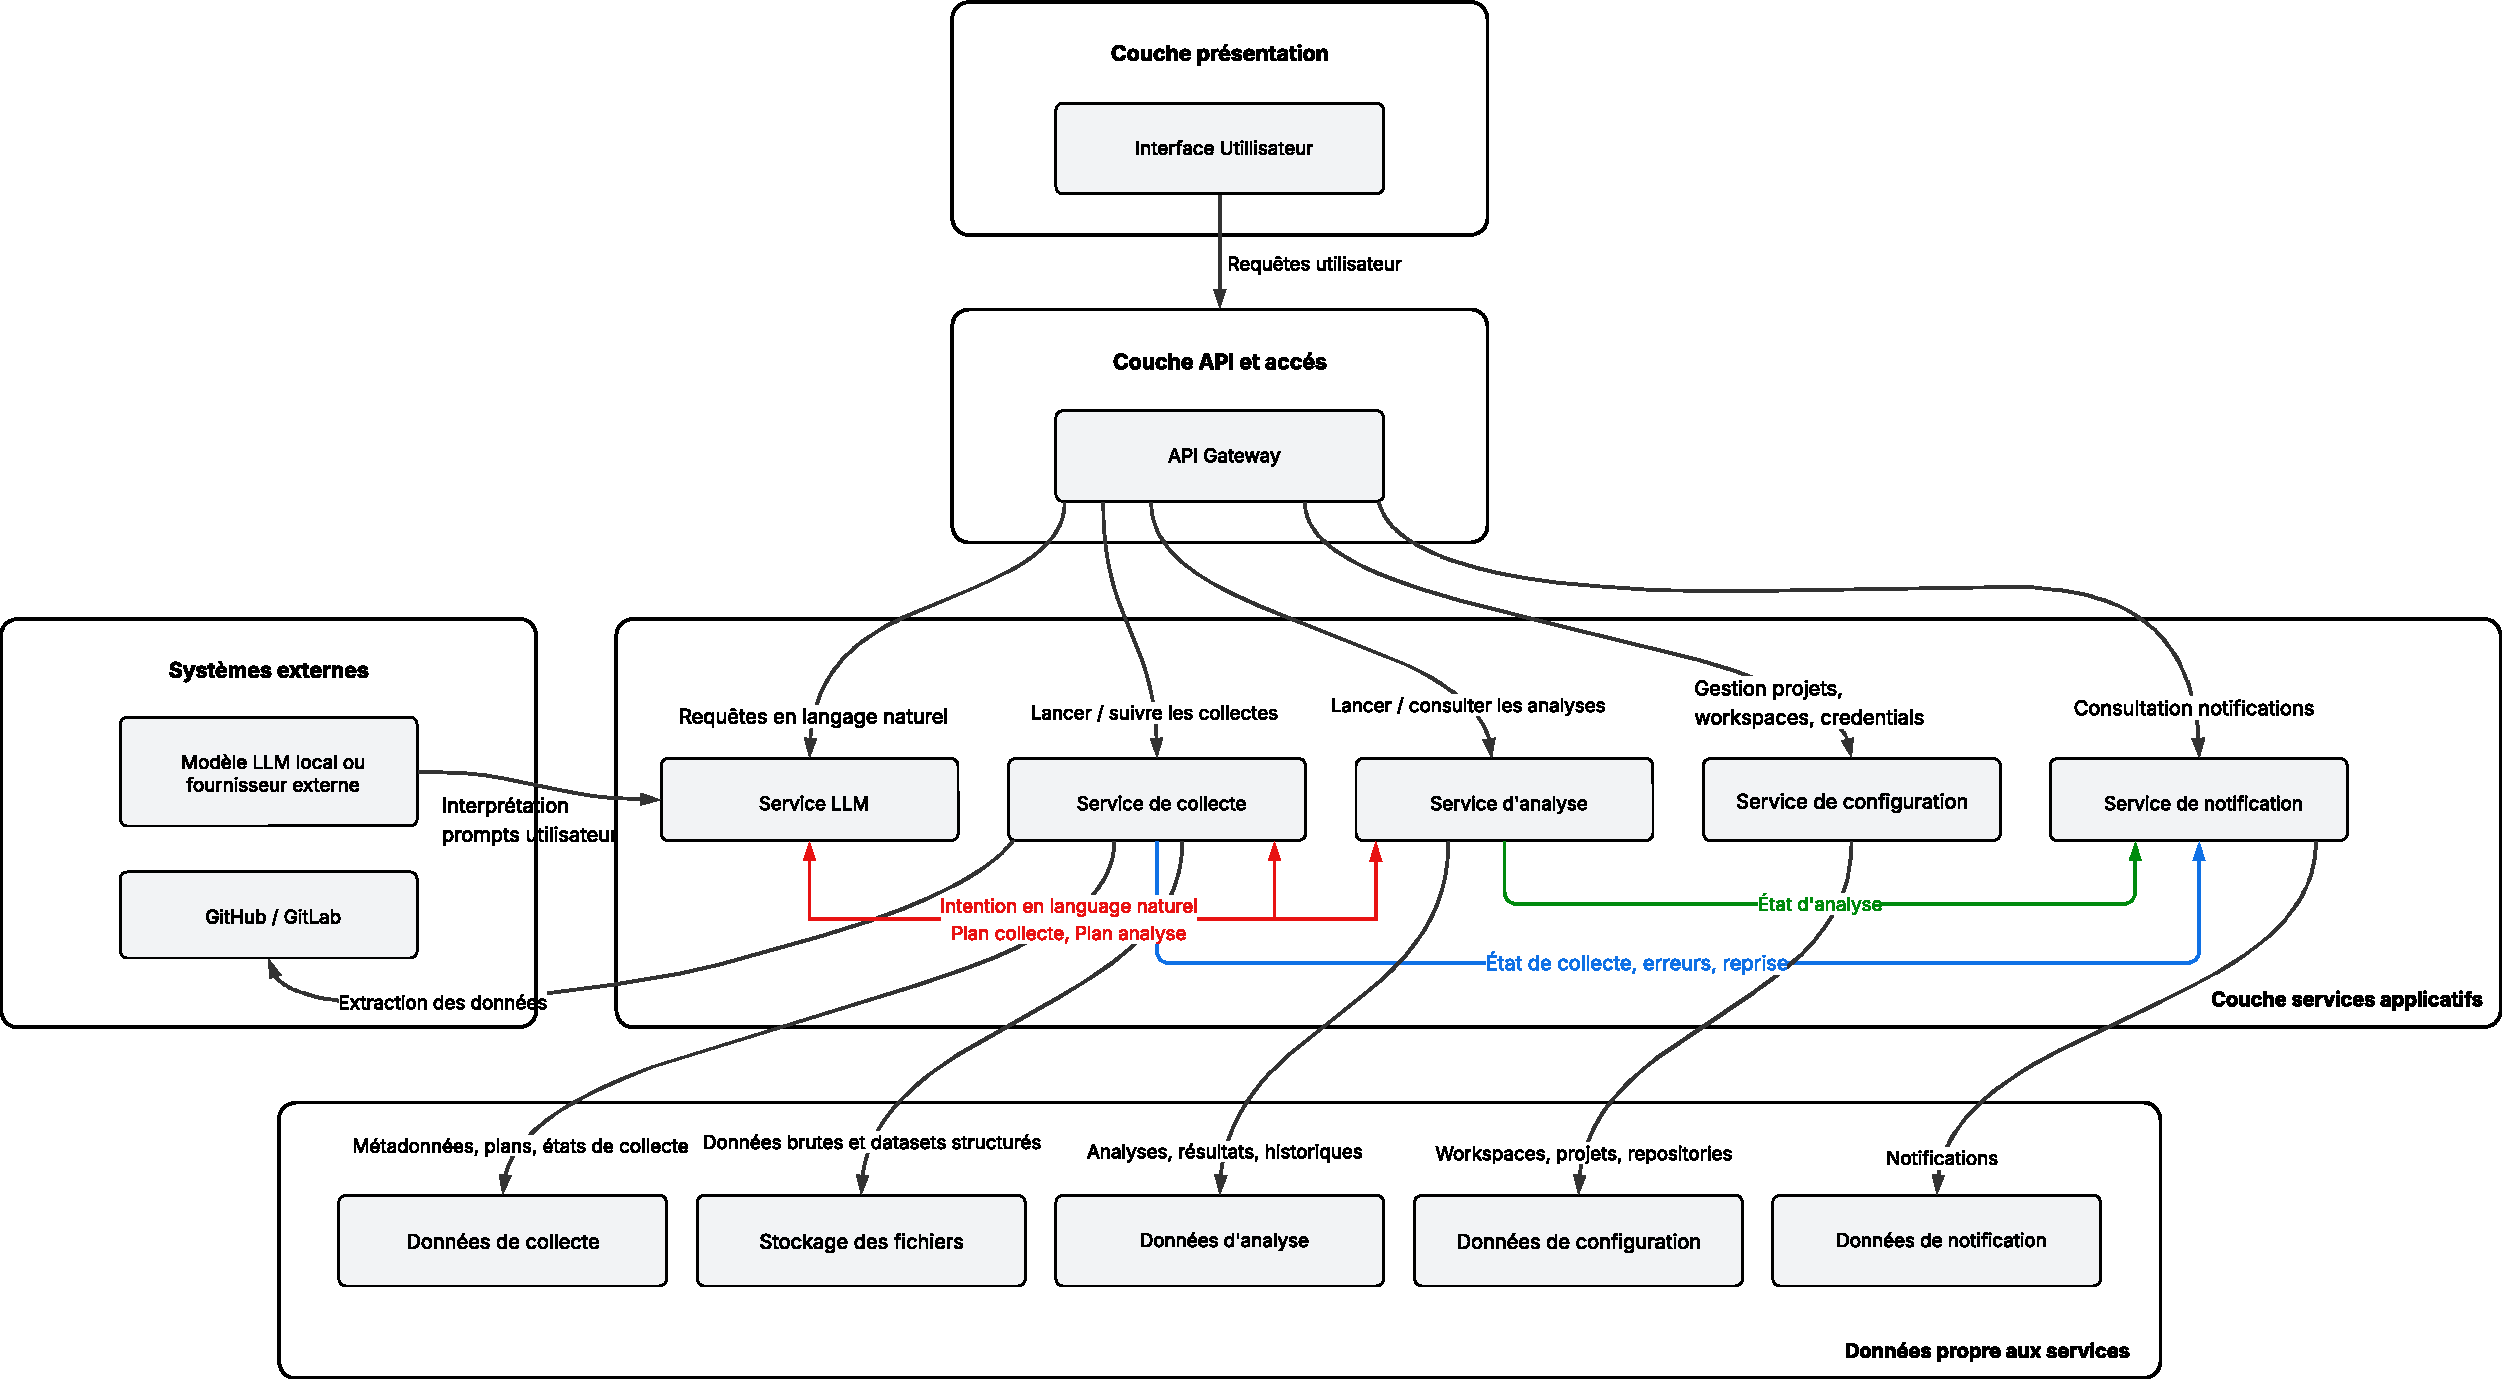
\includegraphics[width=\textwidth]{figures/diagrammComposants.pdf}
    \caption{Vue logique globale des composants de RevMine}
    \label{fig:vue-logique-composants-revmine}
\end{figure}

\section{Conclusion}
Ce chapitre a présenté la conception de la solution RevMine en partant des objectifs définis et des besoins identifiés précédemment. Après une étude comparative des principaux styles architecturaux, nous avons retenu une architecture microservices organisée en couches, adaptée à la séparation des responsabilités, à l’évolutivité et à la maintenabilité de la plateforme.

Nous avons ensuite détaillé la structure globale de RevMine ainsi que la conception interne de ses principaux services, notamment l’API Gateway, le service de configuration, le service de collecte, le service d’analyse, le service LLM et le service de notification.

Ainsi, cette phase de conception établit une base claire pour la mise en œuvre de RevMine, en traduisant les besoins fonctionnels et les choix architecturaux en une structure logicielle cohérente. Le chapitre suivant sera consacré à la réalisation de la solution, où nous présenterons les aspects d’implémentation, les technologies utilisées ainsi que les principales fonctionnalités développées.